\begin{Problem}{Road Construction}{5}

X村内有若干住户。为促进经济发展,方便居民出行,X村准备新修建一条穿城而过的直线形公路。修建的公路必须满足以下条件:

\begin{itemize}
\item 公路不能经过任何住户;
\item 为公平起见,公路两侧的住户数量必须相等;
\item 在满足上述条件的前提下,需要尽量减少交通噪声对居民生活的影响;即,所有住户到公路距离的最小值必须尽可能大。
\end{itemize}

请你帮助X村规划新建的道路。你只需要计算所有住户到公路距离最小值最大能达到多少。

下图是测试数据1的最优道路修建方案。

\begin{figure}[h]
\center
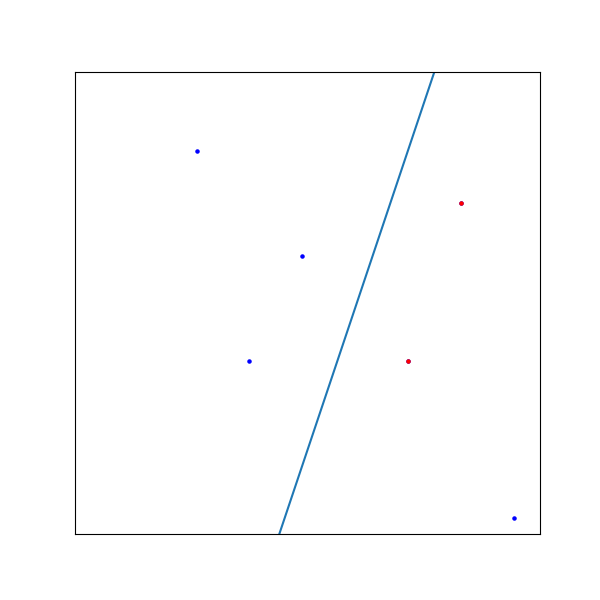
\includegraphics{src/road/01-sample.png}
\end{figure}

\subsection*{输入格式}

第一行包含一个偶数$n$ $(2 \leq n \leq 300)$,表示住户的个数。

接下来$n$行,每行两个整数$x, y$ $(|x|, |y| \leq 10^6)$,表示一个住户的坐标。

保证没有坐标相同的两个住户。

\subsection*{输出格式}

输出一个实数,表示答案。你的答案的绝对或相对误差不应超过$10^{-6}$。

\exmpv{01-sample}
\exmpv{02-sample}

\end{Problem}
